\documentclass{article}

\usepackage{mathrsfs,amsmath}
\usepackage{xcolor}
\usepackage{titlesec}
\usepackage{listings}
\usepackage{syntax}
\usepackage{pythonhighlighting}

\usepackage{graphicx}

\graphicspath{ {./assets/} }

\usepackage[margin=1.4in]{geometry}

\title{Handout \#3 | CS 471} 
\author{Jared Dyreson\\ 
        California State University, Fullerton}

\DeclareRobustCommand{\bowtie}{%
  \mathrel\triangleright\joinrel\mathrel\triangleleft}


\usepackage [english]{babel}
\usepackage [autostyle, english = american]{csquotes}
\MakeOuterQuote{"}

\titlespacing*{\section}
{0pt}{5.5ex plus 1ex minus .2ex}{4.3ex plus .2ex}
\titlespacing*{\subsection}
{0pt}{5.5ex plus 1ex minus .2ex}{4.3ex plus .2ex}

\usepackage{hyperref}
\hypersetup{
    colorlinks,
    citecolor=black,
    filecolor=black,
    linkcolor=black,
    urlcolor=black
}

\begin{document}

\maketitle
\tableofcontents

\newpage

\section{Questions}

\begin{enumerate}

\item Under what conditions are packet delays and losses likely to occur?
\begin{itemize}
\item High volume usage (packet queue is full, therefore cannot accept incoming packets). This results in packet loss.
\item Packets cannot be processed fast enough (packet delay, nothing is lost).
\end{itemize}

\item Assume a circuit switched network based on time division multiplexing. The speed of the link is 1,000 BPS and the size of the single frame is 1 second. The network contains 10 users. All users share the link fairly. How long does it take for a user to transmit a 100,000,000,000 bit file?
\begin{itemize}
\item The link for an individual user would be: $\frac{1000 \text{ bits per second }}{10 \text{ users }} = 100 \text{ bps }$
\item The size of the file is $100,000,000,000$ bits, therefore one user sending this packet would take: $\frac{100,000,000,000}{100} = 1,000,000,000$ seconds
\end{itemize}

\item Assume a network of 100 users. The speed of the shared link is 1,000,000 BPS. Each user is active 5\% of the time. When a user is active, he transmits at a rate of 1,000 BPS.
\begin{itemize}
    \item Circuit switching: $\frac{1,000,000 \text{ bps }}{1,000 \text{ bps }} = 1,000 \text{ simultaneous users }$
\item Packet switching: $\frac{1,000,000 \text{ bps }}{0.05 \times 1000 \text{ bps }} = 20,000 \text{ users }$
\end{itemize}

\item Explain the structure of the contemporary Internet. Be sure to explain the roles of the residential access networks, regional ISPS, tier-1 ISPS, IXPS, peer links and content provider networks.
\begin{itemize}
\item The internet now consists of multiple interconnected large networks.
\item Residential access networks: connects people to the Internet
\item Regional ISPs: an ISP that has subscribers within the franchise area
\item Tier-1 ISPs: Act like global ISPs. These are the networks that are the backbone of the Internet
\item IXPs (Internet Exchange Points): a physical location through which the Internet infrastructure companies such as ISPs and CDNs connect with each other. 
\newpage
\item Peer links: voluntary interconnection of administratively separate Internet networks for the purpose of exchanging traffic between the "down-stream" users of each network.

\begin{figure}[!h]
\centering
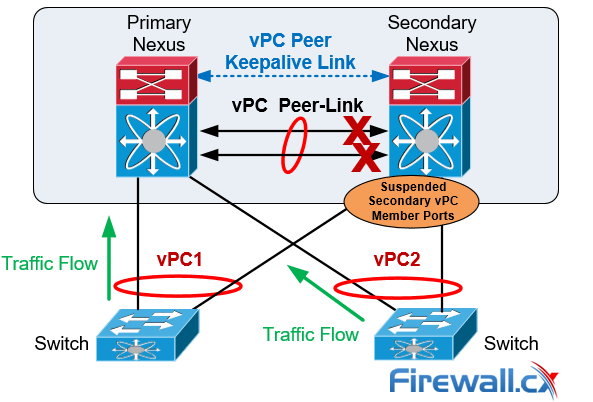
\includegraphics[width=10cm]{peer-link.png}
\caption{Peer Linking}
\end{figure}

\item Content Provider Networks: all companies that operate an Internet Service but do not sell transit within the Peering Ecosystem.

\end{itemize}

\end{enumerate}

\end{document}

